
\section{Communication subsystems}
This section will discuss the  three different communication links to which the emitter satellite is connected:
\begin{itemize}
\item Crosslink for scientific and housekeeping data
\item Ground-space link for scientific data
\item Ground-space link for command and housekeeping data
\end{itemize}

These links are illustrated figure \ref{fig:allesZW}

\begin{wrapfigure}{r}{0.5\textwidth}
\vspace{-60pt}
  \begin{center}
    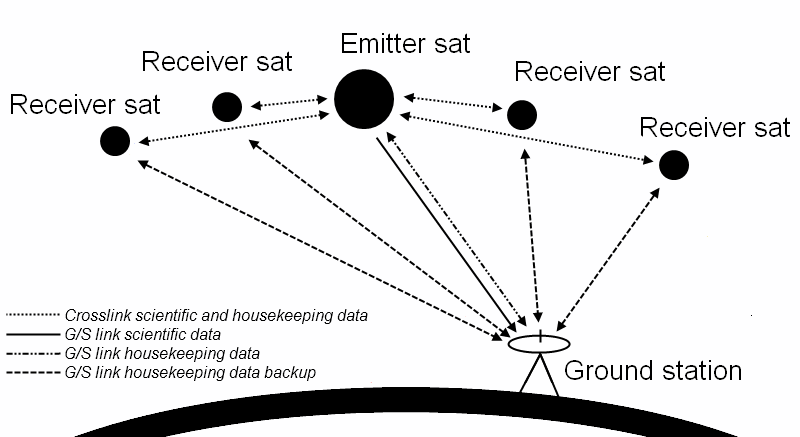
\includegraphics[width=0.48\textwidth]{chapters/img/allesZW.png}
  \end{center}
  \vspace{-15pt}
  \caption{Communications architecture}
  \vspace{-30pt}
  \label{fig:allesZW}
\end{wrapfigure}

For each link the link budget and the communications hardware selected will be presented.

The end of this section contains a piece on the data storage, where the required amount of data storage is found, along with the storage medium to be used and it is checked whether the downlink rate is large enough.


\subsection{Crosslink for scientific data and housekeeping data}
\label{Crossem}
This link transmits the scientific data gathered by the receiver satellites to the emitter satellite. To keep the receiver satellites as small as possible and to have efficient data storage, the receiver satellites will transmit their scientific data continuously so that the emitter satellite can store all data in one data bank before it is transmitted to the ground. In addition to scientific data, command and housekeeping data is also transmitted in this link.

The link budget has the following input parameters: the frequency selected was 2 GHz, the data rate required is 1.62 Mbit/s, the maximum distance between the satellites is 261 km, the modulation used is QPSK. Atmospheric losses were not considered for obvious reasons.

In the mid-term report a frequency in the Ku-band was selected, however it turned out that the data rate was low enough to use S-band or more specifically 2 GHz, which requires far less power consuming hardware.

The maximum distance between two satellites is 261 km, which is longest distance that occurs between the emitter satellite and any of the receiver satellites. Distance between receiver satellites can be twice as long but were not considered after the relative tracking with these crosslinks was abandoned.

The QPSK was selected for its good balance between required E$_{b}$/N$_{0}$ and spectrum utilization. Also a lot of transceivers are available for this modulation.

Another important parameter is the data rate, 1.62 Mbit/s, which was calculated in appendix \ref{scirate}. The position of the satellite is registered every second (144 bits), while for each received photon the coordinates on the array, time, satellite attitude and instrument attitude are registered (295 bits), with 5000 photons expected per second. Adding an extra 10 \% for overhead gives the final data rate between a single receiver satellite and the emitter satellite.


\subsubsection{Transceiver}
\begin{wrapfigure}{r}{0.25\textwidth}
\vspace{-60pt}
  \begin{center}
    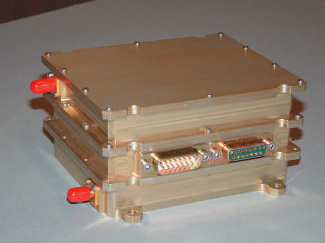
\includegraphics[width=0.24\textwidth]{chapters/img/Strans.png}
  \end{center}
  \vspace{-15pt}
  \caption{S-band tranceiver for microsatellite platforms}
  \vspace{-20pt}
  \label{Strans}
\end{wrapfigure}

Since the data rate is quite high for an S-band, nanosatellite S-band transceivers did not satisfy the requirements, which only allow 9.6 kbps at maximum \cite{cubeshopcomm}. However microsatellite sized transceivers turned out to be sufficient. The transceiver selected was an SBTRcvr of RDLabs, which has a maximum data rate of 10 Mbps for QPSK modulation, an input power of 12 Watt and an output power of 1 to 5 Watt \cite{RDLabs}.


\subsubsection{Antenna}
\begin{wrapfigure}{r}{0.25\textwidth}
\vspace{-20pt}
  \begin{center}
    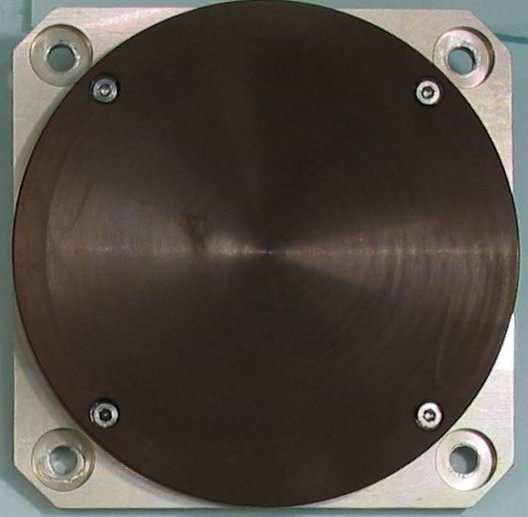
\includegraphics[width=0.24\textwidth]{chapters/img/spatch.png}
  \end{center}
  \vspace{-15pt}
  \caption{S-band patch antenna}
  \vspace{-10pt}
  \label{Spatch}
\end{wrapfigure}
For low gain applications and frequencies below 4 GHz three antennas were considered: a dipole antenna, a helix antenna and a patch antenna. The dipole antenna was not an option since its gain is too low (theoretical gain of a half wave antenna is only 2.15 dBi). A helix antenna would be too large and would decrease the ballistic coefficient too much, for example the S-Band quadrifilar helix antenna of Surrey Satellite technology \cite{SurrHelix} is 0.5 m long with a base of 100mm by 100mm, while the S Band patch antenna \cite{SurrPatch} from the same company is only 20mm thick and 82mm on 82mm large. 
This S Band patch antenna, which was eventually selected, has a mass of only 80 grams, a 120$^{\circ}$ beamwidth and a gain of 4 dBi.
5 antennas will be placed on the emitter satellite: 1 one nadir pointing and 4 facing the receiver satellites.

\subsubsection{Link budget}
Because the selected modulation is QPSK and the maximum allowable bit error rate is 10$^{-5}$, the required E$_{b}$/N$_{0}$ is equal to 9.6 dB. With the output power of the transceiver at maximum (5 Watt or 7 dBW) it is possible to have a E$_{b}$/N$_{0}$ of 10.35 dB, which leaves a margin of 1.76 dB. For detailed link budget see Appendix \ref{linkbudgets}.

\subsection{Ground-space link for scientific data}
As mentioned the past subsection, all scientific data is collected on the emitter satellite which is then transmitted to the ground when it passes its ground station.

The link budget has the following input parameters: the frequency selected was 8.2 GHz, the data rate allowed is 150 Mbit/s, the maximum distance between the ground station and the satellite is 1000 km, the modulation used is QPSK.

The frequency selected is of the X-band as was mentioned in the mid-term review, since it allows a high data rate and is commonly used for Earth observation satellites and thus a lot of ground stations have the right equipment for this frequency band.

The data rate depends on the link time between ground station and satellite, the time between the passes and the storage capacity. The exact required data rate was determined in section \ref{DSEmitter} on data storage and resulted in 111 Mbps, nevertheless the 150 Mbps figure was used in the calculations for the linkbudget to allow for more margin.

The distance between the station and the satellite follows from the maximum beam angle of antenna on the satellite (45$^{\circ}$).

The QPSK modulation was chosen since it also allows a good balance between required E$_{b}$/N$_{0}$ and spectrum utilization and also allows a high data rate of up to 500 Mbps.

\subsubsection{Transmitter}
\begin{wrapfigure}{r}{0.25\textwidth}
\vspace{-50pt}
  \begin{center}
    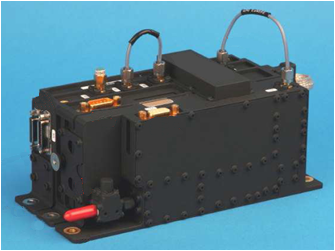
\includegraphics[width=0.24\textwidth]{chapters/img/Xtrans.png}
  \end{center}
  \vspace{-15pt}
  \caption{X-band transceiver XTRA-6}
  \vspace{-40pt}
  \label{Xtrans}
\end{wrapfigure}
The transmitters considered were the XTRA-6 from TESAT Spacecom \cite{TESATxtra} and the HRT150 from General Dynamics and \cite{HRT150}. Since the XTRA-6 is lighter, smaller and requires less power and allows a higher data rate than the HRT150, the choice was quickly made.
The XTRA-6 weighs 1.1 kg, measures 197x89x74 mm, consumes 30 Watts of power and has an output power of 6 Watts.

\subsubsection{Antenna}
\begin{wrapfigure}{r}{0.25\textwidth}[ht]
\vspace{-60pt}
  \begin{center}
    \includegraphics[width=0.24\textwidth]{chapters/img/XPAA.png}
  \end{center}
  \vspace{-15pt}
  \caption{X-band phased array XPAA}
  \vspace{-40pt}
  \label{XPAA}
\end{wrapfigure}
As was chosen in the mid term review, the antenna for the ground space link is a phased array. The phased array selected was the XPAA from Boeing's Phantom works in Seattle \cite{XPAA}. It has a mass of 5.5 kg, measures 330x305x74mm, has a gain of 23.03 dBi and a beamwidth of 15$^{\circ}$.
\subsubsection{Ground station}
The ground station selected was ESRANGE, Kiruna, which allows up to 12 passes a day as it is located above the pole circle. The ground station is operated by ESA and the SSE and is commonly used by Earth observation satellites. For X-band the base has a 13m parabolic receiver dish which has a very high gain, 58 dBi and a beamwidth of 0.18$^{circl}$ \cite{esrange}.

\subsubsection{Link budget}

Similar to the link budget of the crosslinks, the selected modulation is QPSK and the maximum allowable bit error rate is 10$^{-5}$, meaning the required E$_{b}$/N$_{0}$ is equal to 9.6 dB. With the output power of the transceiver at 5 Watt or 7 dBW, it is possible to have a E$_{b}$/N$_{0}$ of 10.35 dB, which leaves a margin of 29.3 dB. For detailed link budget see Appendix \ref{linkbudgets}.

\subsection{Ground-space link for command and housekeeping data}
Aside from the one way space to ground link for scientific data there is also a separate two way link for commands and housekeeping data. 

The link budget has the following input parameters: the frequency selected was 2 GHz, the data rate allowed is 20 kbps, the maximum distance between the ground station and the satellite is 1000 km, the modulation used is QPSK.

The frequency selected is 2 GHz since only a very low data rate is required, and since most ground station over the world are equipped with hardware for S-band links this allows for many contact opportunities to send commands or receive housekeeping data in addition to its main ground station at ESRANGE.

The data rate required is 20 kbps, normally a housekeeping data is never more than a few kbps\cite{satcom} but since the housekeeping data of 5 satellites has to go through the link, it was estimated that 20 kbps should suffice.

The maximum distance is the same as for the space to ground link for scientific data.

The modulation is again QPSK for its balance between required E$_{b}$/N$_{0}$ and spectrum utilization.

\subsubsection{Transceiver}
The transceiver selected was the same as the one used for the crosslinks, the SBTRcvr of RDLabs, as the data required is still too high for nanosatellite transceivers.
\subsubsection{Antenna}
Also the S-band patch antenna from Surrey Satellite technologies was again selected for it small size and sufficient gain.
\subsubsection{Ground station}
The ground station selected was again ESRANGE, Kiruna, for the reasons as the ground-space link for scientific data. For S-band the base has several receiver antennas from 2.4m to 13m, but the linkbudget showed a 2.4m parabolic reflector dish is already more than sufficient. The gain of this antenna is 53 dBi and has a beamwidth of 30$^{circl}$ \cite{esrange}.

\subsubsection{Link budget}
For this last link budget, the selected modulation is QPSK and the maximum allowable bit error rate is 10$^{-5}$, meaning the required E$_{b}$/N$_{0}$ is equal to 9.6 dB. With the output power of the transceiver at 1 Watt or 0 dBW, it is possible to have a E$_{b}$/N$_{0}$ of 39.25 dB, which leaves a margin of 27.65 dB. For detailed link budget see Appendix \ref{linkbudgets}.

\subsection{Data Storage for the Emitter}
\label{DSEmitter}

In order to find an appropriate storage device it is important to known how much data will have to be stored. In order to find this number a ground station is chosen and it is determined when the satellite is in view. Many European polar orbit Earth observation missions use the Kiruna station located close to the North Pole, so the laser swarm will use this station as well. Simulating a period of three weeks will give an indication of when the emitter is in view, the amount of time the satellite is in view and the time in between two passes. The first three entries in table \ref{DSEmitterTable} show the results for these calculations.

Next the total generated bit rate is determined, which is 8.13 [Mbit/s] as indicated in table \ref{DSEmitterTable}. Using this number and the maximum time between two passes over Kiruna the maximum amount of storage required can be determined. The result is indicated in table \ref{DSEmitterTable}, note that a 10\% margin is included to take into account possible anomalies and housekeeping data. 

Now that the required amount of storage is known, a suitable storage device can be chosen. The 64 [Gbit] flash memory module from 3D-Plus \cite{DataStorage} is the best choice due its ability to store a large amount of data in a small, space qualified, package. One module requires about 1 Watt of power and has a weight of 6.10 grams, also it's dimensions are 20.4 x 13.84 x 12.13 mm. Because 244 [Gbit] is required the emitter will be equipped with 5 of these modules. The reason 5 modules are used when 4 would do is to allow for a redundancy in data storage, because it allows more data to be stored should it be required or if one of the other modules malfunctions.

\begin{table}
\centering
\begin{tabular}{c|c}
\textbf{Parameter}  & \textbf{Emitter} \\\hline\hline
	Max. time without contact to ground station & 7:35:33 \\
	Average time without contact to ground station & 1:39:00  \\
	Average duration of contact to ground station & 0:08:30 \\
	Total bit rate [Mbit/s] & 8.13 \\
	Max. amount of data to be stored [Gbit] & 244 \\
	Required downlink rate [Mbit/s] & 111 \\
	Maximum available downlink rate [Mbit/s] & 150 \\
\end{tabular}
\caption{Important values used to determine the required memory for the emitter.}
\label{DSEmitterTable}
\end{table}

Now a suitable storage medium is chosen it is checked whether the stored data can be sent to Earth without running out of storage capacity for new measurements. For the simulated data it is observed that while most of the intervals between contact are about 1,7 hours, and every 13 or more orbits the ground station is not visible for 6 or 7 hours. Taking into account the new data received during these overpasses and the average time the emitter is visible, the resulting required downlink rate is calculated to be 111 [Mbit/s] as indicated in table \ref{DSEmitterTable}. Comparing this with the maximum possible downlink rate it is revealed that the 3D-Plus 64 [Gbit] memory is a viable option. So the emitter will carry 5 x 64 [Gbit] flash memory modules from 3D-Plus for data storage.